\begin{figure}
  \centering
  \begin{subfigure}{0.49\textwidth}
    \centering
    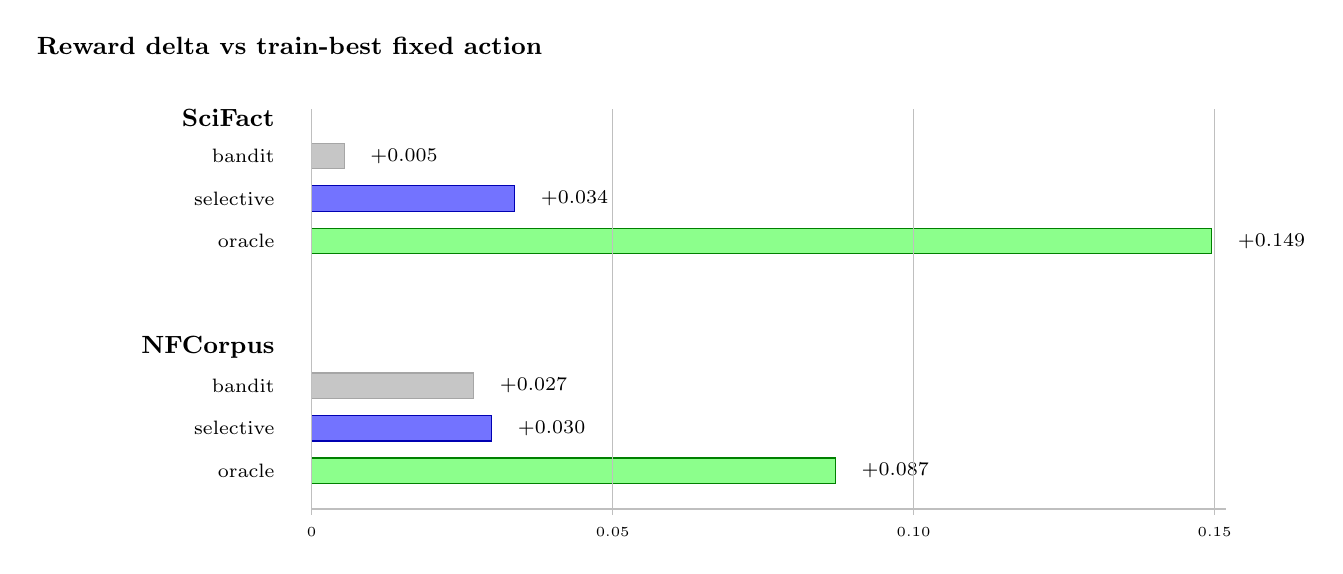
\begin{tikzpicture}[x=1.39cm, y=1.08cm]
      \node[anchor=west, font=\bfseries\small] at (0,6.0) {Reward delta vs train-best fixed action};

      \node[anchor=east, font=\bfseries\small] at (2.35,5.15) {SciFact};
      \node[anchor=east, font=\scriptsize] at (2.35,4.70) {bandit};
      \draw[fill=gray!45, draw=gray!70] (2.60,4.55) rectangle ({2.60+0.0054*55},4.85);
      \node[anchor=west, font=\scriptsize] at ({2.75+0.0054*55},4.70) {+0.005};
      \node[anchor=east, font=\scriptsize] at (2.35,4.20) {selective};
      \draw[fill=blue!55, draw=blue!70!black] (2.60,4.05) rectangle ({2.60+0.0337*55},4.35);
      \node[anchor=west, font=\scriptsize] at ({2.75+0.0337*55},4.20) {+0.034};
      \node[anchor=east, font=\scriptsize] at (2.35,3.70) {oracle};
      \draw[fill=green!45, draw=green!50!black] (2.60,3.55) rectangle ({2.60+0.1495*55},3.85);
      \node[anchor=west, font=\scriptsize] at ({2.75+0.1495*55},3.70) {+0.149};

      \node[anchor=east, font=\bfseries\small] at (2.35,2.45) {NFCorpus};
      \node[anchor=east, font=\scriptsize] at (2.35,2.00) {bandit};
      \draw[fill=gray!45, draw=gray!70] (2.60,1.85) rectangle ({2.60+0.0269*55},2.15);
      \node[anchor=west, font=\scriptsize] at ({2.75+0.0269*55},2.00) {+0.027};
      \node[anchor=east, font=\scriptsize] at (2.35,1.50) {selective};
      \draw[fill=blue!55, draw=blue!70!black] (2.60,1.35) rectangle ({2.60+0.0299*55},1.65);
      \node[anchor=west, font=\scriptsize] at ({2.75+0.0299*55},1.50) {+0.030};
      \node[anchor=east, font=\scriptsize] at (2.35,1.00) {oracle};
      \draw[fill=green!45, draw=green!50!black] (2.60,0.85) rectangle ({2.60+0.0870*55},1.15);
      \node[anchor=west, font=\scriptsize] at ({2.75+0.0870*55},1.00) {+0.087};

      \draw[black!25] (2.60,0.55) -- (10.95,0.55);
      \foreach \x/\lab in {2.60/0,5.35/0.05,8.10/0.10,10.85/0.15} {
        \draw[black!25] (\x,0.48) -- (\x,5.25);
        \node[font=\tiny, anchor=north] at (\x,0.45) {\lab};
      }
    \end{tikzpicture}
    \caption{Reward-delta ladder}
  \end{subfigure}
  \hfill
  \begin{subfigure}{0.47\textwidth}
    \centering
    \begingroup
    \setlength{\fboxsep}{0.45em}
    \fbox{
      \begin{minipage}{0.86\textwidth}
        \centering
        \textbf{\Large Defense Numbers}\\[0.55em]
        \small
        \begin{tabular}{@{}lcc@{}}
          \toprule
          \textbf{Metric} & \textbf{SciFact} & \textbf{NFCorpus} \\
          \midrule
          Selective reward $\Delta$ & +0.0337 & +0.0299 \\
          Gap closed & 22.6\% & 34.4\% \\
          Constrained utility $\Delta$ & +0.0474 & +0.0327 \\
          Selective calls/query & 1.413 & 1.000 \\
          3-seed win & 0.667 & 0.667 \\
          \bottomrule
        \end{tabular}

        \vspace{0.6em}
        \raggedright
        \textbf{CI evidence:} reward CIs stay above zero on both datasets; utility CIs are +0.0143 to +0.0822 and +0.0106 to +0.0584.
      \end{minipage}
    }
    \endgroup
    \caption{Numeric readout}
  \end{subfigure}

  \caption{Primary visual evidence: selective-policy gains plus readable cost-aware and robustness diagnostics.}
\end{figure}
